\section{Principal Queries}
%\textcolor{red}{[Write some of the queries to be performed to satisfy your functional requirements. 3-4 queries are enough, try to use the techniques seen at lecture (aggregate functions, group by, subqueries,…)]}


\lstset{language=SQL,
keywordstyle=\color{blue},
stringstyle=\color{mauve},
showstringspaces=false,
breaklines=true,
commentstyle=\color{orange}\ttfamily,
basicstyle=\ttfamily\footnotesize}

\begin{itemize}
\item Finding the information about the customers who have a package on the way, the day when the package is created and the shipping company which is delivering it
\lstinputlisting[frame=single]{sections/queries&more/q1.sql}
The output is shown below.\\ 
\vspace{0.2cm}\\
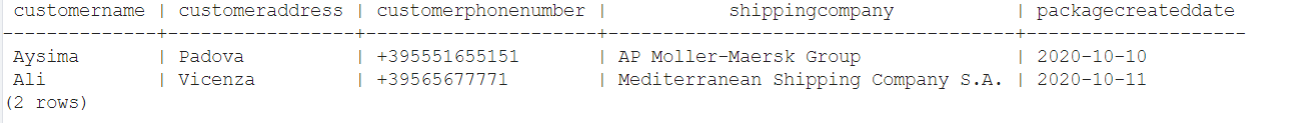
\includegraphics[width=0.9\textwidth]{sections/queries&more/q1.png}

\item Finding the Copy{\_}ID, ISBN and the warehouse address where the Copy that is inside a package was stored
\lstinputlisting[frame=single]{sections/queries&more/q2.sql}
The output is shown below.\\ 
\vspace{0.2cm}\\
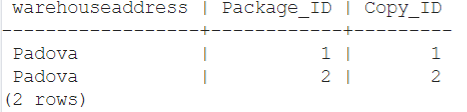
\includegraphics[width=0.9\textwidth]{sections/queries&more/q2.png}

\item Finding the customers who have sent a message, the message that they have sent, and the admin who has received it
\lstinputlisting[frame=single]{sections/queries&more/q3.sql}
The output is shown below.\\ 
\vspace{0.2cm}\\
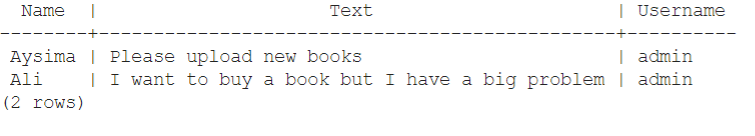
\includegraphics[width=0.8\textwidth]{sections/queries&more/q3.png}

\item Find the authors who have written programming books which are stored in the database and the titles of the books they have written
\lstinputlisting[frame=single]{sections/queries&more/q4.sql}
The output is shown below.\\ 
\vspace{0.2cm}\\
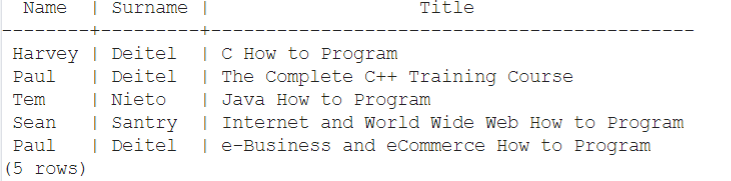
\includegraphics[width=1\textwidth]{sections/queries&more/q4.png}

\item Find the number of copies each book has and display all the information about each book
\lstinputlisting[frame=single]{sections/queries&more/q5.sql}
The output is shown below.\\ 
\vspace{0.2cm}\\
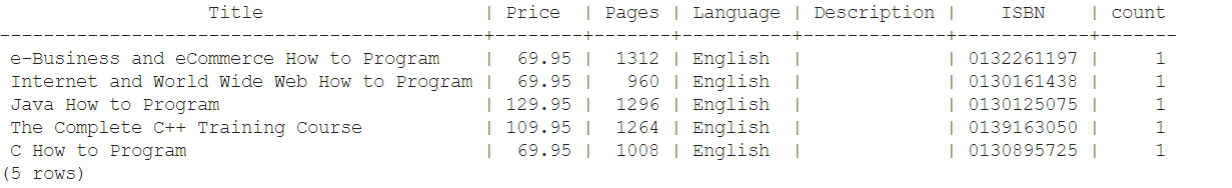
\includegraphics[width=1\textwidth]{sections/queries&more/q5.png}
\end{itemize}